\begin{figure}[htb]
\captionsetup[subfigure]{font={bf,large}, skip=1pt, margin=-0.7cm,justification=raggedright, singlelinecheck=false}
\centering
  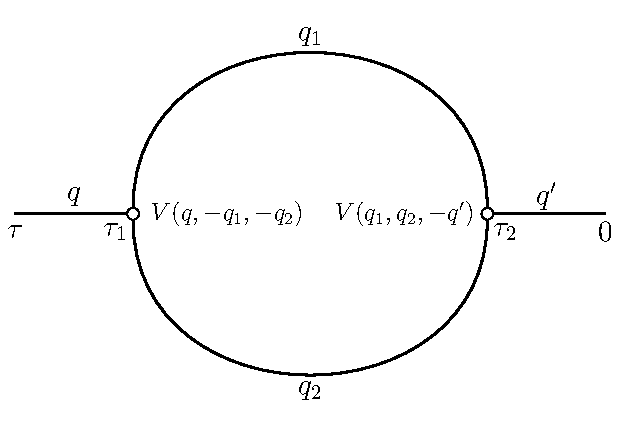
\includegraphics[width=0.5\textwidth]{fig_3_2_bubble/bubble_explain.pdf}
  \caption{The one of the lowest order ($\lambda^2$) diagram of phonon-phonon interactions of \cref{173254_31Jan24} in the imaginary time space. Starting from the right at $\tau=0$, the free phonon line with $q'$ goes to the $V(q_{1},q_{2},q')$ vertex at $\tau=\tau_{2}$, which splits into two free phonons with $q_{1}$ and $q_{2}$. They gather at the $V(q, q_{1},q_{2})$ vertex at $\tau=\tau_{1}$, and the free phonon with $q$ reaches $\tau$.}

\label{Fig:diagram:example}
\end{figure}